\documentclass[UTF8]{ctexart}
\usepackage{graphicx}

\title{%
  试使用控制论方法\\设计广州大学教学质量控制系统\\
  \large 第3小组 Week4}

\author{
谢金宏 \and 胡涛 \and 何汉根 \and 房华恒
\and 奚厚铧 \and 李俊民 \and 陈淇铭 \and 陈树康
}

\begin{document}

\maketitle

\section{整体设计}

\begin{figure}[htbp]
	\centering
	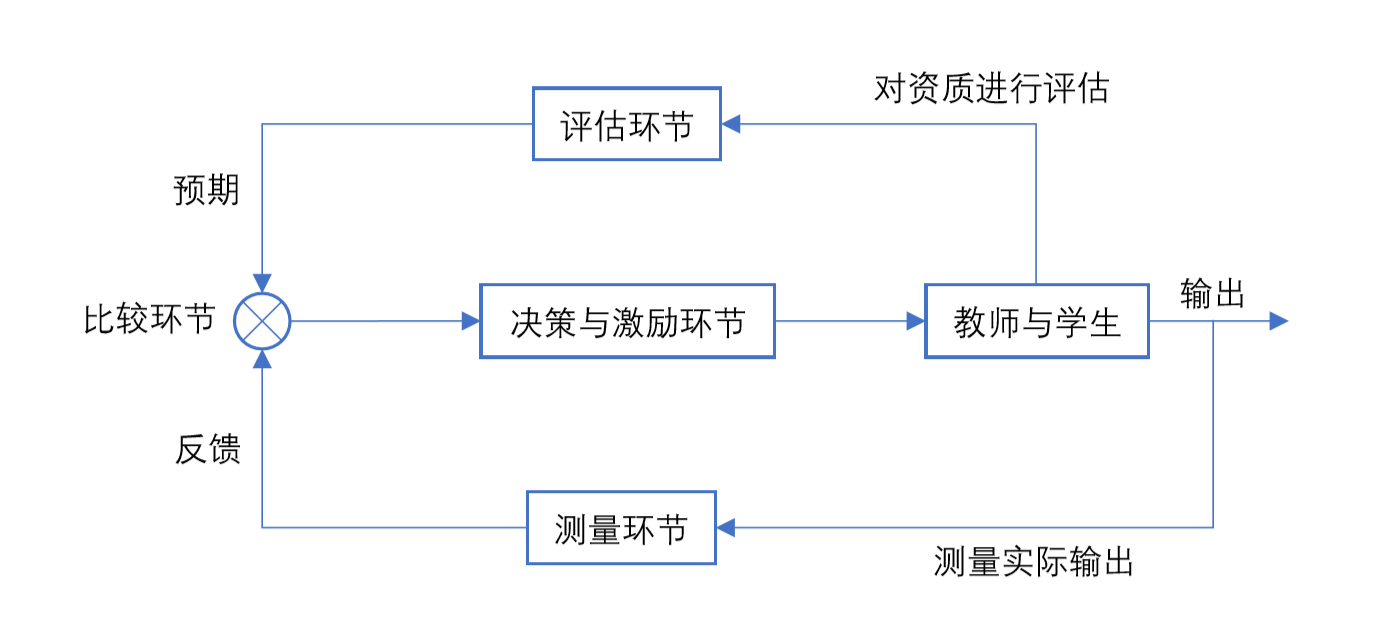
\includegraphics[width=\linewidth]{images/week4-design.png}
	\caption{整体设计图}
\end{figure}

上图展示了我们小组设计的广州大学教学质量控制系统的主要组成要素。在该系统中,受控对象为老师和学生,主要的环节有:评估环节、测量环节、比较环节、决策与激励环节。

\section{教师与学生}

教师与学生是系统中的受控对象,我们关心受控对象与教学方面相关的信息。具体地讲,对于教师,我们关心教师的职称、在其他教师中的声誉、在学生中的口碑、教师的教学风格等;对于学生,我们关于高考成绩、过往校内学习成绩等。

上述的信息在教师入职和学生入学时收集,并通过评估环节和测量环节不断更新,实现信息的新陈代谢。

\section{评估环节}

我们对教学质量的评估的粒度细化到课程。对于某一具体的课程,我们考虑教学质量的量化指标有出勤率、课程成绩(包括平时成绩和考试成绩)、课堂活跃程度等。

在“教师与学生”一节中我们收集了教师与学生的相关信息,而在当前环节,我们利用这些信息和其他附加信息(如学生的专业与所选课程的相关程度等),通过算法(采用一次函数模型),产生教学质量评估的量化指标的一个期望值。

\section{测量环节}

测量环节贯穿课程的始末,是对我们提出的量化指标的测量。对于出勤率、课堂活跃程度等指标,我们可以采用课堂监控摄像和人脸识别技术来实现信息的自动化收集。对于学生的课程成绩指标,我们可以要求教师及时提交相关材料。与教师相关的测量则由学生通过课程评价网站进行。学生可以在课程评价网站上对教师进行点评打分,给教师打标签,评价其教学方式。

\section{比较、决策和激励环节}

通过比较评估环节中得出的量化指标的期望值和测量环节中的测量值可以得出理想情况与真实情况的差距。当实际指标低于我们的期望时,可以决策通过一些措施来激励教师或学生。学生的激励可以采用调整奖学金的金额和名额分配等方式进行;教师的激励可以采用根据学生反馈调整教师工资、调整学生反馈在教师职称评定中的影响力等方式进行。

\end{document}
